\chapter{Calibration of the DORI Prototype}
\section{Energy Calibration}
\label{sec:energy_calibration}
As a novel approach for PSs, the energy response was calibrated using the \emph{Bremsstrahlung} endpoint of an X-ray tube. The maximum X-ray photon energy produced corresponds to the scenario in which the accelerated electron transfers all its kinetic energy in a single interaction with the anode nucleus. The maximum energy detected, i.e., the endpoint of the acquired spectrum, is therefore equal to the tube voltage, which serves as the energy reference for calibration. Since the \emph{Bremsstrahlung} spectrum near the endpoint is approximately linear, this abscissa can be determined as the $x$-intercept of a least-squares fit to that region~\cite{121}. This test and all subsequent tests relying on X-ray production used an Apogee 5500 Series tube (Oxford Instruments). It is 50~W tube that operates over a voltage range of 0 to 50~kV, with a maximum beam current of 1.0~mA~\cite{oxford2019apogee}.

The detector was positioned in the beam line, at a distance sufficient to avoid saturation of the front-end electronics. \emph{Bremsstrahlung} spectra were acquired over 5-minute intervals for tube voltages of 15--50~kVp and tube currents of 0.050--0.250~mA, and are shown in Fig.~\ref{fig:bremss_calibration} (a) and (b), respectively. Background was subtracted, and channels 18 and below were again excluded. As represented in Fig.~\ref{fig:bremss_calibration} (a), the 15~kVp spectrum is not visible, as it sits within the excluded background. At this distance and fluence, photons of such low energy are absorbed by the black adhesive tape used for light-wrapping of the photosensitive detector element. This establishes the lower bound of the calibrated range at 20~keV.
\begin{figure}[H]
  \centering
  \begin{minipage}[c]{0.48\linewidth}
    \centering
    \subfloat[]{\label{fig:bremss_spectra}%
      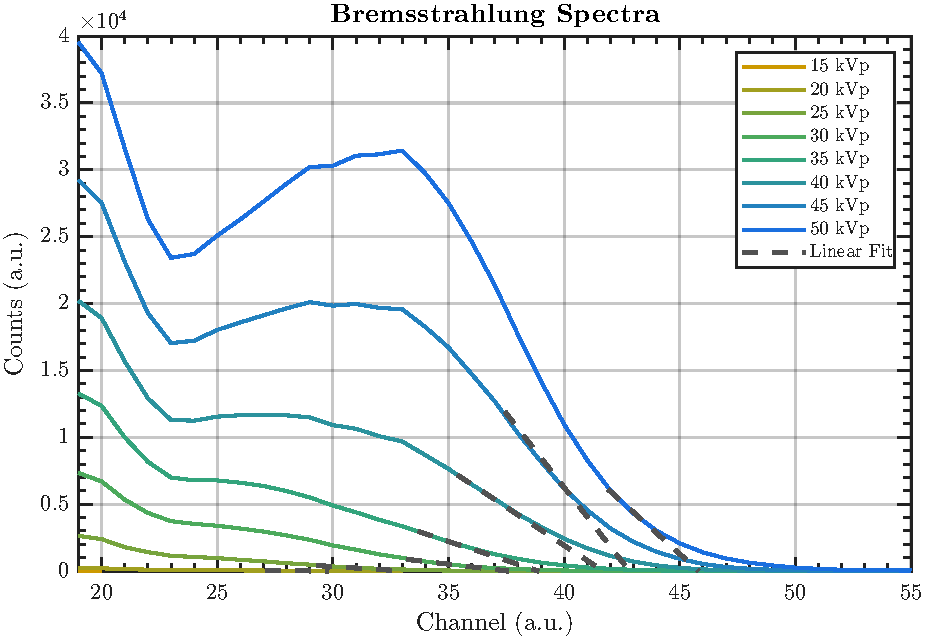
\includegraphics[width=\linewidth]{images/bremsstrahlung_fits.pdf}}
  \end{minipage}%
  \hfill%
  \begin{minipage}[c]{0.48\linewidth}
    \centering
    \subfloat[]{\label{fig:bremss_endpoint}%
      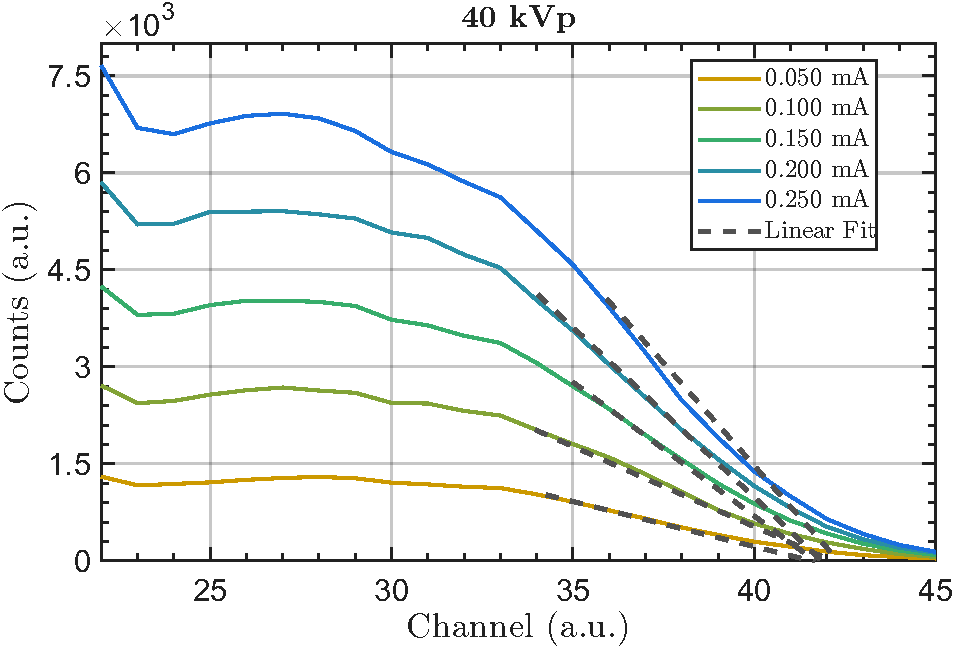
\includegraphics[width=\linewidth]{images/bremsstrahlung_40kVp_vs_current.pdf}}
  \end{minipage}
  \caption[\emph{Bremsstrahlung} Spectra.]{%
    \emph{Bremsstrahlung} spectra, background subtracted and excluded;
    \textbf{(a)} acquired at 0.250~mA for tube voltages from 15 to 50~kVp;
    \textbf{(b)} acquired at 40~kVp for tube currents from 0.050 to 0.250~mA.
  }
  \label{fig:bremss_calibration}
\end{figure}

The linear region of each \emph{Bremsstrahlung} spectrum was selected interactively, and a least-squares regression was applied to the points within that window. The $x$-intercept of the fitted line gives the endpoint channel. Since tube current affects only photon fluence and not the spectral endpoint, the five acquisitions per voltage produce five independent estimates (see Fig.~\ref{fig:bremss_calibration} (b)). The resulting values are summarized in Table~\ref{tab:endpoints}.

% Small vertical space after surrounding text
\vspace{1em}

% Manual table title, numbered and added to LoT
\refstepcounter{table}
\label{tab:endpoints}
\noindent\textbf{Table~\thetable.} \emph{Bremsstrahlung} endpoint channel for each tube voltage. Values are the mean of five acquisitions with the maximum deviation from the mean.
\addcontentsline{lot}{table}{\protect\numberline{\thetable}\emph{Bremsstrahlung} endpoint channel for each tube voltage.}

% Small space between title and table
\vspace{0.1em}

\begin{table}[H]
  \centering
  \begin{tabular}{>{\centering\arraybackslash}m{0.18\textwidth}
                  >{\centering\arraybackslash}m{0.08\textwidth}
                  >{\centering\arraybackslash}m{0.08\textwidth}
                  >{\centering\arraybackslash}m{0.08\textwidth}
                  >{\centering\arraybackslash}m{0.08\textwidth}
                  >{\centering\arraybackslash}m{0.08\textwidth}
                  >{\centering\arraybackslash}m{0.08\textwidth}
                  >{\centering\arraybackslash}m{0.08\textwidth}}
    \toprule
    \scriptsize \textbf{Tube Voltage (kVp)} & \scriptsize \textbf{20} & \scriptsize \textbf{25} & \scriptsize \textbf{30} & \scriptsize \textbf{35} & \scriptsize \textbf{40} & \scriptsize \textbf{45} & \scriptsize \textbf{50} \\
    \midrule
    \scriptsize \textbf{Endpoint Channel (a.u.)}
    & \scriptsize $31 \pm 3\%$
    & \scriptsize $33 \pm 3\%$
    & \scriptsize $37 \pm 1\%$
    & \scriptsize $39 \pm 1\%$
    & \scriptsize $42 \pm 1\%$
    & \scriptsize $43 \pm 1\%$
    & \scriptsize $45 \pm 2\%$ \\
    \bottomrule
  \end{tabular}
\end{table}
Although 20 and 25 keV lie in the boundary at which photoeletric absorption ceases to dominate in BC-408 (see Appendix~B), the associated uncertainty is dominated by counting statistics. The associated error improves between 30 and 45 keV, indicating that in this region both the photoelectric cross-section and the photon fluence are sufficient for the endpoint to be determined with good precision. At 50 keV, the photoelectric absorption in the scintillator drops below 0.5\%, and consequently the uncertainty increases. As full energy transfer becomes less probable, the spectrum compresses toward a lower and less reliable endpoint. Additionally, pileup further distorts the spectral shape near the abscissa. The pileup distortion is visible as a non-linear tail in the higher energy spectra of Fig.~\ref{fig:bremss_calibration} (a), which is not characteristic of filtered \emph{Bremsstrahlung}. At higher count rates, the baseline does not recover between successive pulses, causing them to superimpose and producing the observed tail. These are the fundamental limitations of the endpoint method at higher energies, as the associated uncertainty is expected to grow accordingly.

To extend the calibration beyond the range of the X-ray tube, spectra of the reference sources were acquired with the PS five times, each over a 90 min interval. Of the three sources, the only features available are the $^{241}$Am photopeak at 59.5 keV, and the CE of the 122 keV line of $^{57}$Co, at 39.46 keV, shown in Fig.~\ref{fig:source_spectra} (a) and (b) respectively. 
\begin{figure}[H]
  \centering
  \begin{minipage}[c]{0.50\linewidth}
    \centering
    \subfloat[]{\label{fig:Am-241}%
      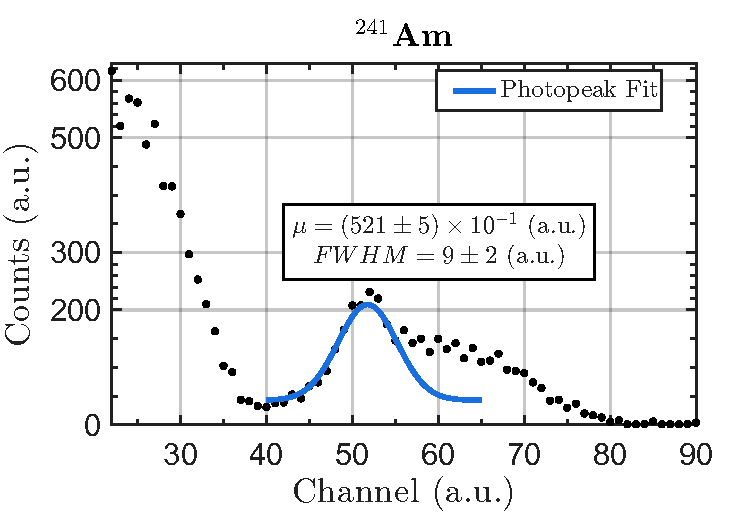
\includegraphics[width=\linewidth]{images/plastic_Am-241.pdf}}
  \end{minipage}%
  \hfill%
  \begin{minipage}[c]{0.50\linewidth}
    \centering
    \subfloat[]{\label{fig:Co-57}%
      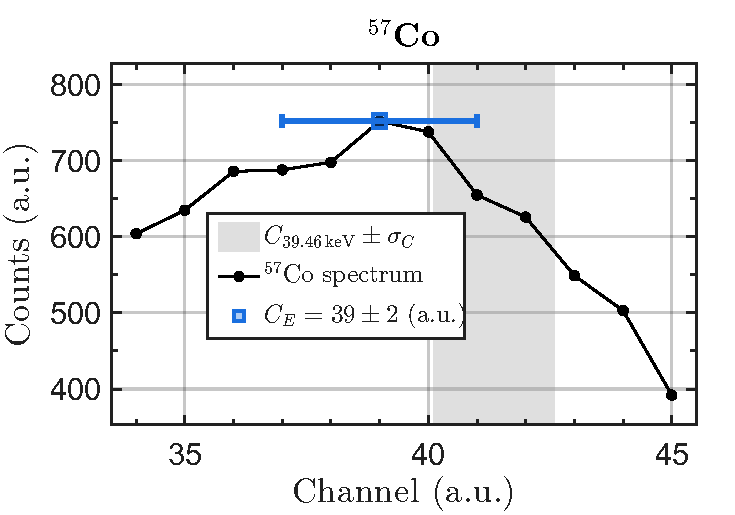
\includegraphics[width=\linewidth]{images/plastic_Co-57_fit.pdf}}
  \end{minipage}
  \caption[Reference source spectra.]{%
    Reference source spectra, background subtracted. Annotated values are the mean of five acquisitions with the maximum deviation from the mean as uncertainty.
    \textbf{(a)} $^{241}$Am, with the Gaussian fit to the 59.5~keV photopeak.
    \textbf{(b)} $^{57}$Co's Compton Edge at 39.46~keV.
  }
  \label{fig:source_spectra}
\end{figure}

The $^{241}$Am photopeak is fully resolved and was described by a Gaussian fit, whereas the $^{57}$Co CE was extracted as the channel of maximum counts. Despite the lower number of counts accumulated in the photopeak, it has the smaller uncertainty of the two features, and although it is not as sharp as the one obtained with the CsI crystal in Section~\ref{sec:frontend-validation}, the centroid position is reproducible across acquisitions. The broadening of the $^{57}$Co feature is a consequence of the energy dependence of the resolution and its degradation at lower energies. The photopeak is therefore included as a calibration point at 59.5~keV, whereas the edge, falling within the interval already covered by the tube, is treated as an independent validation of the \emph{Bremsstrahlung} method.

A weighted least-squares fit was applied to account for the differences in uncertainty across the energy range and is shown in Fig.~\ref{fig:energy_calibration}.
\begin{figure}[H]
  \centering
  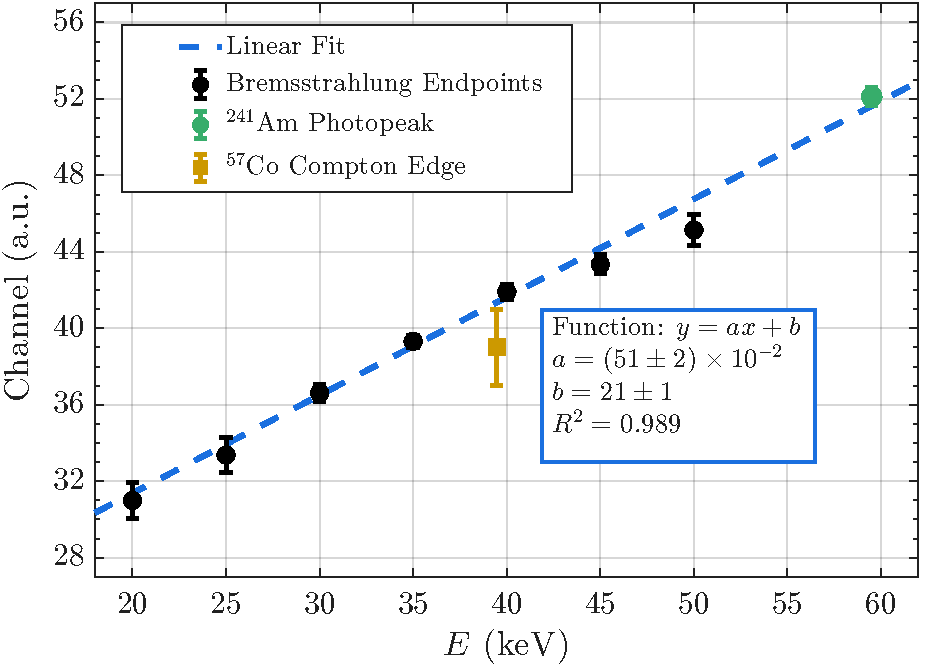
\includegraphics[width=0.85\linewidth]{images/energy.pdf}
  \caption[Energy calibration of the DORI prototype.]{%
    Weighted least-squares energy calibration of the DORI prototype, obtained from the seven \emph{Bremsstrahlung} endpoints and the $^{241}$Am photopeak centroid. The $^{57}$Co Compton edge is superimposed for validation.
  }
  \label{fig:energy_calibration}
\end{figure}
Although the 45 keV uncertainty is small, both the 45 and 50 keV endpoints fall below the calibration line, beyond their uncertainties. This underestimation is consistent with the compression of the spectrum discussed above. In contrast, the $^{241}$Am centroid falls on the calibration line with an uncertainty smaller than that of the highest-energy endpoint estimate. The weighted fit ensures that these better-determined points contribute more to the calibration, and the uncertainties in each estimate propagate into the calibration coefficients~\cite{121}. The fit is of the form:
\begin{equation}
    C = aE + b,
    \label{eq:calibration}
\end{equation}
where $C$ is the channel number and $E$ is the energy in keV. With $R^2 = 0.989$, the DORI response can be treated as locally linear within the calibrated interval of 20 to 60 keV. Given a measured channel, the energy is therefore obtained from the following simplified expression~\cite{125}:
\begin{equation}
    E = \frac{C - 21}{0.51},
    \label{eq:energy_conversion}
\end{equation}
\begin{equation}
    \sigma_E = \frac{1}{0.51}\sqrt{(0.02)^2\,E^2 + 1^2}.
    \label{eq:energy_uncertainty}
\end{equation}


The $^{241}$Am photopeak in Fig.~\ref{fig:source_spectra} (a) has a FWHM of $9 \pm 2$ channels, above the minimum of five channels set in Section~\ref{sec:shaping}. The chosen gain therefore samples the photopeak adequately. As the only available photopeak, its centroid is also used to calculate the energy resolution of the DORI system at 59.5 keV. Although $R$ is dimensionless and, in principle, independent of the channel-to-energy conversion, the non-zero intercept $b$ shifts the centroid without contributing to the FWHM. Consequently, the resolution differs between channel and energy space and these parameters must be converted to energy using Eqs.~\ref{eq:energy_conversion} and \ref{eq:energy_uncertainty}. With these values, DORI has an energy resolution of $R = (29 \pm 5)$\% at 59.5 keV, consistent with values reported in the literature, and previously discussed, for BC-408 PSs. 

As for the CE of the 122~keV line of $^{57}$Co, the extracted channel falls below the calibration line, outside of it even within its own uncertainty. This discrepancy was predicted in Section~\ref{sec:scintillator} and is attributed to the extraction method rather than to the calibration itself. According to Swiderski~\emph{et al.}~\cite{127}, the finite resolution of PSs causes the channel of maximum counts not to coincide with the true position of the edge. The CE lies at a channel above that of maximum counts, and the offset grows as the resolution degrades. Taking CE as the maximum of the distribution therefore introduces a systematic and observed underestimation. The deviation is thus not evidence of a failure of the \emph{Bremsstrahlung} calibration, although the extraction method does not allow it to be validated either. Additionally, extension of the linear fit to 100 keV cannot be assumed, as it would span the non-proportional region of the plastic response discussed in Section~\ref{sec:scintillator}. In the absence of additional calibration points, the gap between 60 and 100 keV is acknowledged as a limitation of the present calibration. Within these limits, the DORI prototype response across the 20 to 60 keV range is characterized and the following dose calibration is performed within this interval.

\section{Dose Calibration}
\label{sec:dose_rate_calibration}

As introduced, an individual monitoring device is calibrated in personal dose equivalent, $H_p(d)$, with $d = 10$~mm adopted, the depth at which the quantity is defined for whole-body exposure. These devices are calibrated in certified laboratories, which have reference instruments and ensure the reproducibility and traceability of the measurements. The available reference fields include radionuclide sources, mono-energetic X-radiation and continuous filtered X-ray beams of defined quality, and conversion coefficients are provided for all of them. The calibration presented here follows the ISO 4037 series~\cite{113,ISO2,ISO3} for the conversion of \emph{air KERMA} to $H_p(10)$, using filtered X-ray beams of the narrow (N) series, the same reference qualities over which the commercial RaySafe i3 is calibrated. The protocol was adapted to the instrumentation available with the intention of demonstrating the methodology and showing that DORI can be calibrated as a prototype.

\subsection{Setup}
The production of the radiation quality needed depends on the tube potential, the total filtration and the properties of the anode. Given the X-ray tube available and the energy calibration, only radiation qualities with energies in the 20 to 50~keV range can be used. In the N-series that corresponds to N-25, N-30 and N-40, as the N-20 spectrum falls outside the calibrated energy range. The parameters defining each of the three qualities, together with the corresponding conversion coefficients, are listed in Table~\ref{tab:nseries}.
% Small vertical space after surrounding text
\vspace{1em}

% Manual table title, numbered and added to LoT
\refstepcounter{table}
\label{tab:nseries}
\noindent\textbf{Table~\thetable.} N-series radiation qualities. Coefficients correspond to the ISO slab phantom at 1-meter normal incidence. Adapted from Refs.~\cite{113,ISO3}.%
\addcontentsline{lot}{table}{\protect\numberline{\thetable}N-series radiation qualities.}

% Small space between title and table
\vspace{0.1em}

\begin{table}[H]
  \centering
  \begin{tabular*}{\textwidth}{@{\extracolsep{\fill}}cccc@{}}
    \toprule
    \textbf{\begin{tabular}[b]{@{}c@{}}Radiation\\Quality\end{tabular}} &
    \textbf{\begin{tabular}[b]{@{}c@{}}Tube Potential\\(kVp)\end{tabular}} &
    \textbf{\begin{tabular}[b]{@{}c@{}}Added\\Filtration\end{tabular}} &
    \begin{tabular}[b]{@{}c@{}}$\bm{h_{pK}(10)}$\\\textbf{(Sv/Gy)}\end{tabular} \\
    \midrule
    \textbf{N-25} & 25 & 2 mm Al & 0.574 \\
    \textbf{N-30} & 30 & 4 mm Al & 0.815 \\
    \textbf{N-40} & 40 & 4 mm Al + 0.21 mm Cu & 1.210 \\
    \bottomrule
  \end{tabular*}
\end{table}
As introduced, the dosimeter must be placed on a PMMA phantom during the calibration. For $H_p(10)$ the ISO water slab phantom is used, since it reproduces the backscatter of the trunk of the body and therefore the conditions under which the dosimeter is worn for this specific quantity. It consists of a PMMA shell of 30 $\times$ 30 $\times$ 15~cm, with a 2.5~mm front wall and 10~mm remaining walls, filled with water~\cite{ISO3}. A phantom replicating these dimensions was built for this work, but it was not filled with water, due to the risk of leakage in the presence of electronics around the setup. The DORI-test board was taped to the front wall of the phantom, with its photosensitive area aligned with the centre of the tube. Custom 3D-printed supports were made to hold the filters, and these sit on an alignment rail together with the phantom. The setup is shown in Fig.~\ref{fig:setup}. The centre of the PS entrance face is placed 1~meter away from the tube, and this position is taken as the reference measurement point, marked by the red star in the image. The \emph{air KERMA} was measured with the R/F Low detector of the RaySafe Xi~\cite{raysafe}, which was the only one to provide a measurable signal at this distance. The instrument was last calibrated in October 2013 and the product has since been discontinued, however, it was the only reference available. For these measurements the phantom and the dosimeter are removed from the rail and the centre of the R/F Low detector is placed at the reference point. 

It should be noted that the reference conditions under which the conversion coefficients of Table~\ref{tab:nseries} are defined cannot be fully reproduced with the available instrumentation. The phantom was not filled with water, so the backscatter contribution is lower than the one assumed by the standard. The anode is made of molybdenum instead of tungsten, although its characteristic lines lie below the calibrated energy range and therefore do not contribute to the measured spectra. The inherent filtration falls only within the maximum deviation permitted by ISO 4037, and the HVL of each quality were not tracked. Most importantly, the main limitation is the reference instrument itself. The values obtained are therefore not traceable and the procedure described here does not constitute a formal calibration. Its purpose is to establish and validate a methodology that reproduces the ISO 4037 framework as closely as the available setup allows, so that the same procedure can later be planed and repeated at a certified facility under the required field conditions. 
\begin{figure}[H]
  \centering
  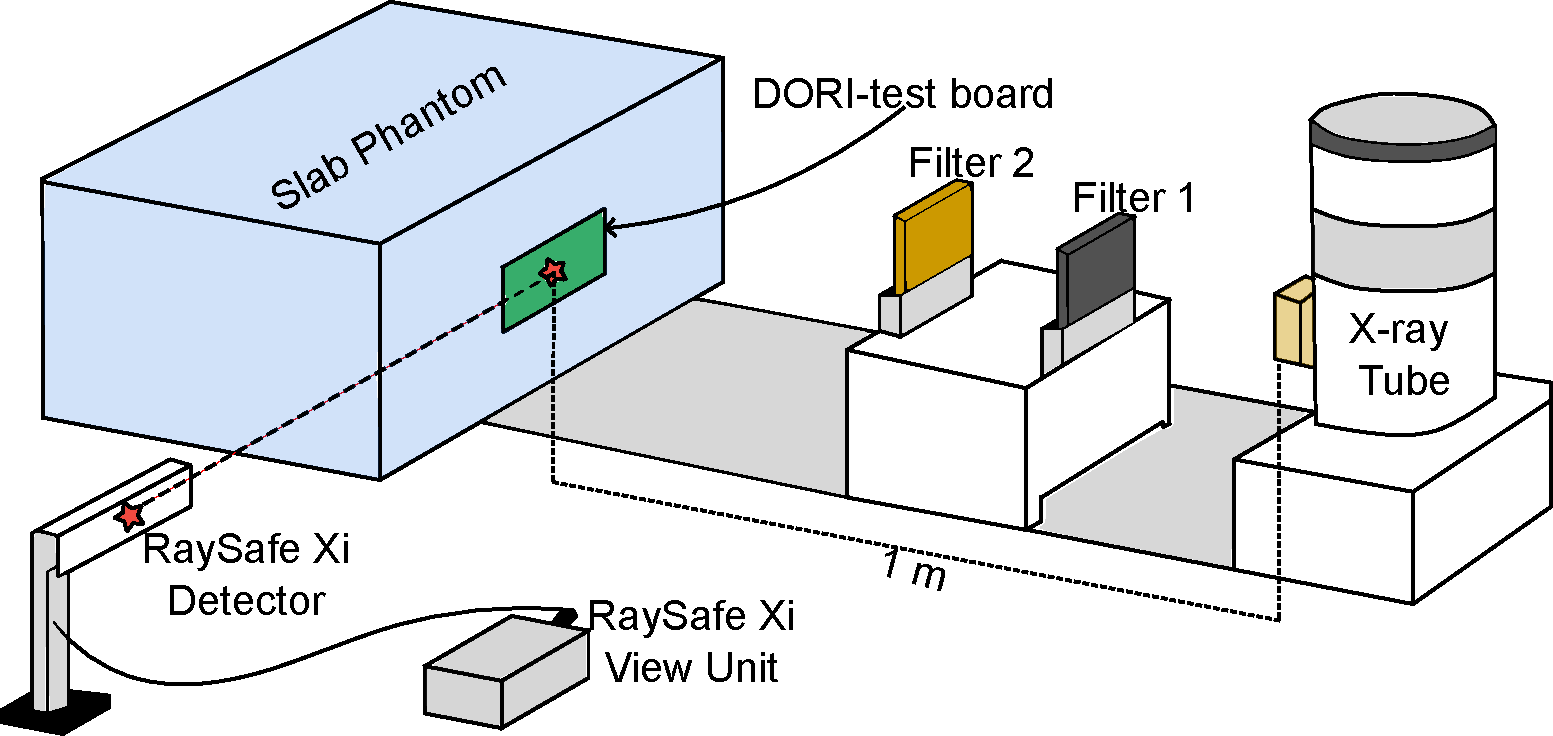
\includegraphics[width=\linewidth]{images/dose.pdf}
  \caption[Dose calibration setup.]{Dose calibration setup. The beam quality is defined by the placement of one filter, or two in the case of N-40, at the exit window of the X-ray tube. The DORI-test board is placed at the reference measurement point (red star), in contact with the front wall of the built slab phantom. The RaySafe Xi detector is positioned at the same point of test free in air, with the phantom removed, and the \emph{air KERMA} values are read on its view unit.}
  \label{fig:setup}
\end{figure}



All acquisitions were made at a tube current of 0.5~mA for 2 minutes, and the spectrum and average \emph{air KERMA} rate from DORI and the RaySafe were recorded, respectively.
The spectra acquired are shown in Fig.~\ref{fig:dose}~(a). Counts below the lower limit of the validated energy calibration and above the endpoint energy of the respective beam were excluded. Each spectrum is therefore confined to its expected energy range, and noise and pile-up events are rejected.

\begin{figure}[H]
  \centering
  \begin{minipage}[c]{0.50\linewidth}
    \centering
    \subfloat[]{\label{fig:dose_spectra}%
      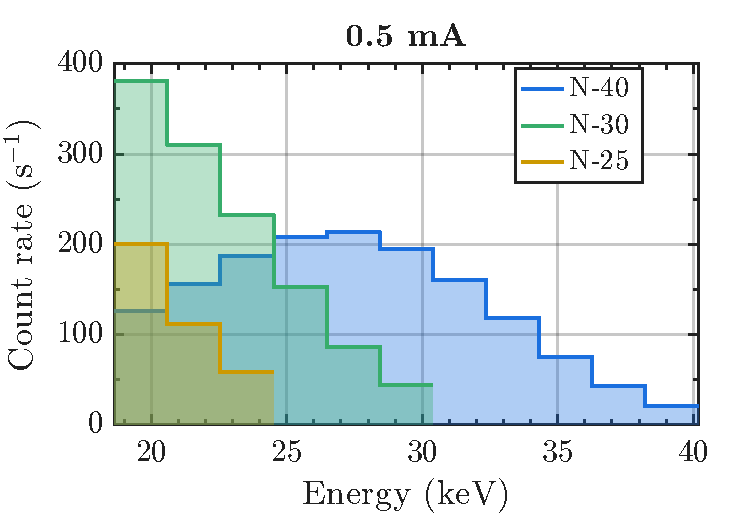
\includegraphics[width=\linewidth]{images/fig1_spectra.pdf}}
  \end{minipage}%
  \hfill%
  \begin{minipage}[c]{0.50\linewidth}
    \centering
    \subfloat[]{\label{fig:hp_10}%
      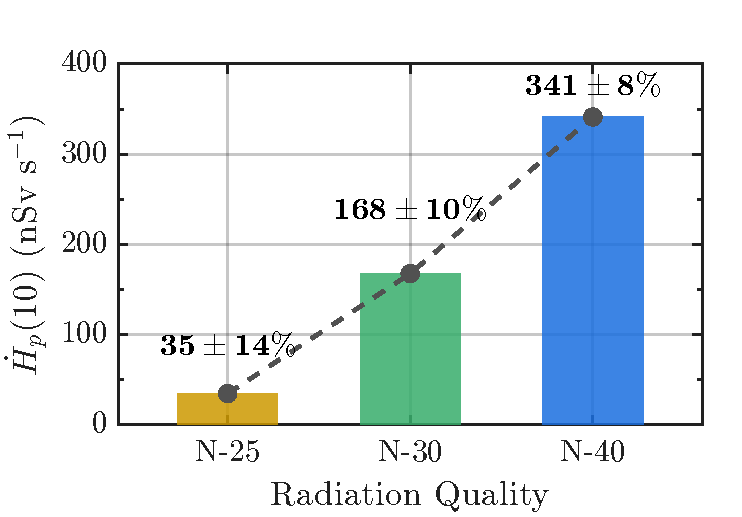
\includegraphics[width=\linewidth]{images/fig2_reference.pdf}}
  \end{minipage}
  \caption[ISO 4037 narrow-series qualities N-25, N-30 and N-40, acquired at 0.500~mA for 2 minutes.]{ISO 4037 narrow-series qualities N-25, N-30 and N-40, acquired at 0.500~mA for 2 minutes.
    \textbf{(a)} Energy spectra;
    \textbf{(b)} reference $\dot{H}_p(10)$.
  }
  \label{fig:dose}
\end{figure}

The effect of the filtration can be seen, since all acquisitions were made at the same tube current and for the same duration. Without filtration, the count rate would scale approximately with the square of the tube potential. The N-series filtration is designed to narrow the spectrum by suppressing its low-energy component. The lower count rate registered at the lower energies for N-40 is a direct consequence of the copper filter. This is not seen for N-30. N-30 requires twice the aluminium of N-25 and yet exceeds it at every energy the two share, since the higher output of the harder beam compensates the additional attenuation. The low-energy component of N-40 is nevertheless not completely suppressed. The detected counts originate from Compton interactions in the PS and from photons scattered by the slab phantom, which is itself intended to produce scattering. As a consequence, the mean energy of each distribution falls progressively below the value tabulated by ISO for the corresponding quality.

The reference $\dot{H}_p(10)$ obtained for each quality is shown in Fig.~\ref{fig:dose}(b), calculated from the measured \emph{air KERMA} rate and the conversion coefficients of Table~\ref{tab:nseries}. The values increase with tube potential, as both terms of the product grow with beam energy. The relative uncertainty decreases with tube potential, from $14\%$ at N-25 to $8\%$ at N-40. The \emph{air KERMA} rates of N-30 and N-40 sit above the trigger level of the detector ($>100$~nGy~s$^{-1}$)~\cite{Specs}, while that of N-25 is flagged as a low signal, contributing to the higher uncertainty.

\subsection{Methods}

The absorbed dose increases with the energy deposited, so counts registered at different energies do not produce the same biological effect. $H_p(10)$ can therefore be written as a sum over the spectrum, each count contributing according to the energy at which it was detected:
\begin{equation}
H_p(10) = \sum_{i=1}^{m} w_i N_i ,
\label{eq:bin_model}
\end{equation}
where $N_i$ is the number of counts and $w_i$ the dose per count, in Sv/count.  Each weight holds the response of DORI to the ISO reference field in that energy range, since it converts the counts the device registers into the dose delivered. Calibrating the dosimeter in dose therefore corresponds to determining the set of weights $w_i$.
 
As shown, each radiation quality produces one pulse height spectrum with an associated $H_p(10)$ rate. Since the radiation is not monoenergetic, the weights cannot be assigned to individual energies. The spectrum must instead be grouped into $m$ bins, each covering a range of energies which will carry the same weight. The number of bins that can be resolved is limited by the number of radiation qualities available, as each quality provides one equation of the form of Eq.~\ref{eq:bin_model}. For $q$ radiation qualities, the measurements can be written as:
\begin{equation}
\begin{bmatrix}
H_1 \\ H_2 \\ \vdots \\ H_q
\end{bmatrix}
=
\begin{bmatrix}
N_{11} & N_{12} & \cdots & N_{1m} \\
N_{21} & N_{22} & \cdots & N_{2m} \\
\vdots & \vdots  & \ddots & \vdots \\
N_{q1} & N_{q2} & \cdots & N_{qm}
\end{bmatrix}
\begin{bmatrix}
w_1 \\ w_2 \\ \vdots \\ w_m
\end{bmatrix},
\label{eq:system}
\end{equation}
where each row of $\mathbf{A}$ holds the counts per bin measured for one quality, $\mathbf{H}$ is the measured $H_p(10)$ and $\mathbf{w}$ the unknown weights. For $q > m$ the system is overdetermined and is solved by the least-squares method~\cite{portable}:
\begin{equation}
\mathbf{w} = \left(\mathbf{A}^{\!\top}\mathbf{A}\right)^{-1}
\mathbf{A}^{\!\top}\mathbf{H} .
\label{eq:lsq}
\end{equation}

With three radiation qualities available, $q = 3$ and the system of Eq.~\ref{eq:system} admits at most three unknowns. Solving it with $m = 3$ fits the three measurements exactly, leaving no redundancy with which to verify the solution and making no use of the uncertainties of the reference values. Choosing $m = 2$ leaves one degree of freedom, which allows a weighted solution and leaves a residual against which the quality of the fit can be assessed. For this case, the counts of every quality are summed into two groups separated by a single boundary. Eleven channels cover the 20 to 40~keV range, so ten boundary positions are possible. All of them were tested and the two most representative cases are shown in Fig.~\ref{fig:weights}~(a) and (b), the division at 25~keV and the equal-width division at 30~keV, respectively.

\begin{figure}[H]
  \centering
  \begin{minipage}[c]{0.48\linewidth}
    \centering
    \subfloat[]{\label{fig:w_2bin25}%
      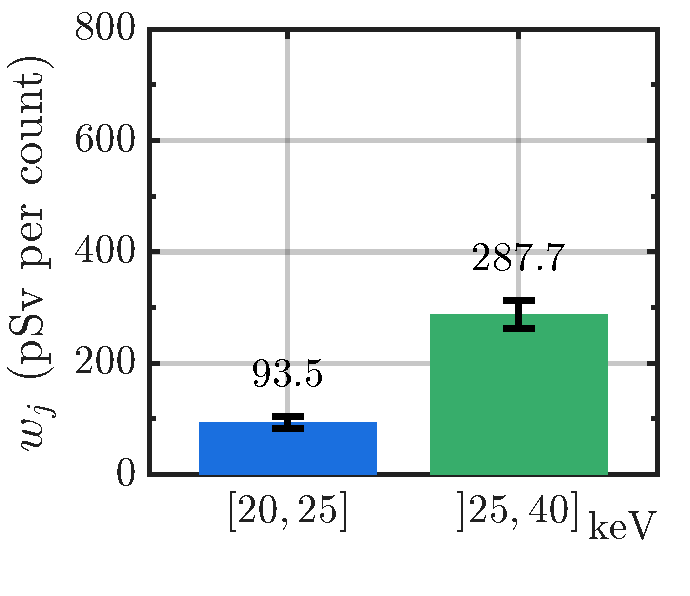
\includegraphics[width=\linewidth]{images/weights2bin25_sub.pdf}}
  \end{minipage}%
  \hfill%
  \begin{minipage}[c]{0.48\linewidth}
    \centering
    \subfloat[]{\label{fig:w_2bin30}%
      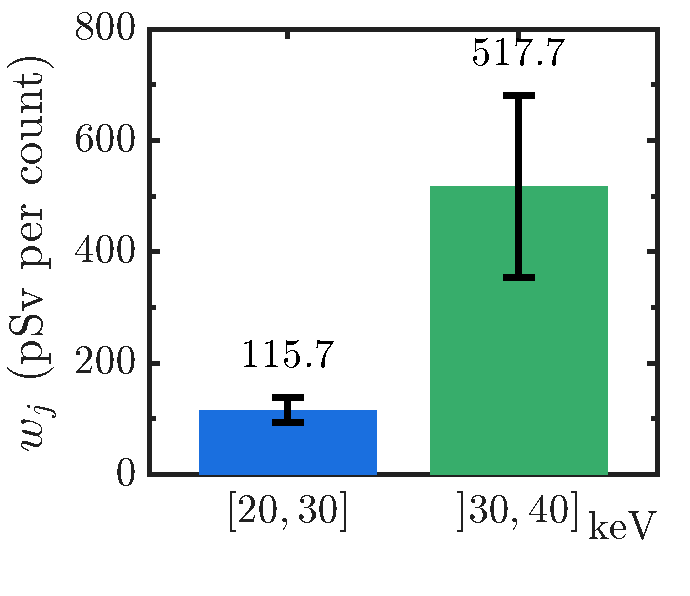
\includegraphics[width=\linewidth]{images/weights2bin30_sub.pdf}}
  \end{minipage}

  \vspace{1em}
  \begin{minipage}[c]{0.85\linewidth}
    \centering
    \subfloat[]{\label{fig:w_3bin}%
      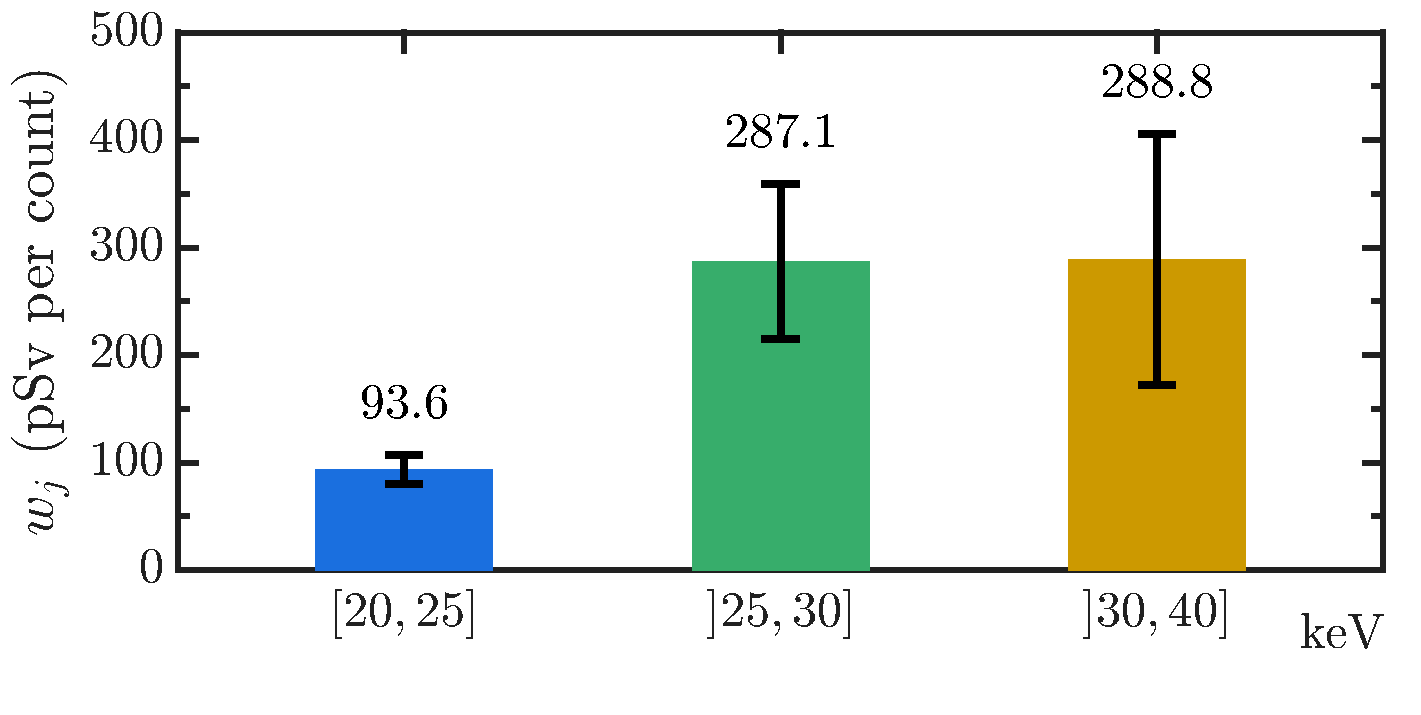
\includegraphics[width=\linewidth]{images/weights3bin_sub.pdf}}
  \end{minipage}
  \caption[Dose per count obtained for three binning schemes.]{Dose per count obtained for three binning schemes within the calibrated 20 to 40~keV range.
    \textbf{(a)} Two bins divided at 25~keV;
    \textbf{(b)} two bins divided at 30~keV;
    \textbf{(c)} three bins divided at 25 and 30~keV.
  }
  \label{fig:weights}
\end{figure}


Both divisions return $w_2 > w_1$, as expected from the increase of dose with the energy detected, but they differ in how well each weight is determined. At 25~keV the boundary coincides with the end of the N-25 spectrum. N-25 therefore falls entirely in the lower bin and fixes $w_1$ by itself, while N-30 and N-40 both populate the upper bin and together determine $w_2$. Every quality is used, and the uncertainties obtained are the lowest of the three schemes. For any boundary above this energy, N-25 and N-30 both contribute to the lower bin, and for these cases, most notably at 30~keV, the two qualities have incompatible values of $w_1$, $93.6$ and $139.0$~pSv/count respectively. The solution is therefore a compromise between the two. Additionally, and as represented for this specific scenario, the uncertainty of $w_2$ is the largest, which makes this division unsuitable.

The small number of measurements also allows the solution to be determined directly. As mentioned in the last paragraph, since N-25 has no counts in the upper bin, it determines $w_1$ on its own, $93.6 \pm 13.2$~pSv/count. Subtracting that contribution from N-30 gives $w_2 = 287.1 \pm 72.0$~pSv/count over the 25 to 30~keV range, and subtracting both contributions from N-40 gives $w_3 = 288.8 \pm 116.9$~pSv/count over the 30 to 40~keV range. Two independent radiation qualities therefore return the same weight, within the uncertainty of the fit, and the increase expected for the third weight is marginal and lies only within its uncertainty. This reasoning is the three-bin solution represented in Fig.~\ref{fig:weights}~(c). For this scenario, the uncertainties of the two upper weights increase to $25\%$ and $40\%$ against $10\%$ in the two-bin solution, which makes the model less robust.

A two-bin model was therefore adopted, with $N_1 \in \left[20,25\right]$~keV and $N_2 \in \left]25,40\right]$~keV, and Eq.~\ref{eq:bin_model} reduces to:
\begin{equation}
H_p(10) = w_1 N_1 + w_2 N_2 ,
\label{eq:two_bin}
\end{equation}
with the values in Fig.~\ref{fig:weights}~(a):
\begin{equation}
w_1 = 93.5 \pm 11.4, \qquad w_2 = 287.7 \pm 25.5,\ \text{unit: } \left[\frac{\mathrm{pSv}}{\mathrm{count}}\right] .
\label{eq:weights}
\end{equation}
 
\noindent A count registered in the upper bin therefore carries $3.1$ times the dose of a count registered in the lower bin, which translates the effect of higher energy on the dose delivered. It should be noted that a 15~keV bin is broad considering the available range, but it is again a consequence of the small number of radiation qualities that can be used. A tube capable of higher potentials would provide additional qualities and allow finer divisions. Given a measured spectrum, the personal dose equivalent is therefore obtained from the following simplified expression:
\begin{equation}
    H_p(10) = 93.5\,N_1 + 287.7\,N_2 ,
    \label{eq:dose_conversion}
\end{equation}
\begin{equation}
    \sigma_{H_p(10)} = \sqrt{\left(11.4\,N_1\right)^2 + \left(25.5\,N_2\right)^2} ,
    \label{eq:dose_uncertainty}
\end{equation}

The response of DORI after calibration is shown in Table~\ref{tab:response}, where the reconstructed ${H}_p(10)$ agrees with the reference value within the uncertainty, for the three qualities and for both reconstructions. The calibration therefore reproduces the measurements from which it was derived. Additionally, a leave-one-out test was performed, where the weights are recomputed from two qualities and used to predict the $\dot{H}_p(10)$ of the third by reconstructing the dose from its own bin counts. The most interesting result is the case of N-25. As mentioned, it is the only direct measurement of $w_1$. When excluded, $w_1$ can only be inferred from the different proportions in which N-30 and N-40 divide their counts between the two bins. As can be seen, the reconstructed dose differs by approximately $0.3\%$, indicating that $w_1$ is well determined by the available measurements and is not an artefact of the single quality that defines it.

Overall, these results support the two-bin model and the position of its boundary, and indicate that, with the three measurements available, this was the best division that could be made. The precision of the calibration is limited not only by the number of qualities, but also by the uncertainty of the reference dose values, which is dominated by the RaySafe Xi for the reasons already given. It should be emphasised that a formal calibration was never the purpose. The goal of demonstrating that a prototype of this kind can be calibrated in dose from its own spectrum has been achieved, and the methodology is shown to be workable. A significant part of the future work will therefore be to extend the energy calibration to higher energies and to obtain more reliable $\dot{H}_p(10)$ reference values.

\vspace{1em}
\refstepcounter{table}
\label{tab:response}
\noindent\textbf{Table~\thetable.} Reference $\dot{H}_p(10)$ and the values reconstructed by the two-bin calibration and by the leave-one-out test, for the three radiation qualities.
\addcontentsline{lot}{table}{\protect\numberline{\thetable}Response of DORI after the dose calibration.}

\vspace{0.1em}
\begin{table}[H]
  \centering
  \begin{tabular*}{\textwidth}{@{\extracolsep{\fill}}cccc@{}}
    \toprule
    \textbf{\begin{tabular}[b]{@{}c@{}}Radiation\\Quality\end{tabular}} &
    \textbf{\begin{tabular}[b]{@{}c@{}}Reference\\(nSv s$^{-1}$)\end{tabular}} &
    \textbf{\begin{tabular}[b]{@{}c@{}}Calibration\\(nSv s$^{-1}$)\end{tabular}} &
    \textbf{\begin{tabular}[b]{@{}c@{}}Leave-one-out\\(nSv s$^{-1}$)\end{tabular}} \\
    \midrule
    \textbf{N-25} & $35 \pm 5$   & $35 \pm 4$  & $35 \pm 8$ \\
    \textbf{N-30} & $168 \pm 16$ & $168 \pm 13$ & $168 \pm 14$ \\
    \textbf{N-40} & $341 \pm 26$ & $341 \pm 27$ & $340 \pm 75$ \\
    \bottomrule
  \end{tabular*}
\end{table}




\section{Dose Rate Reconstruction}
\label{sec:dose_rate}

The spectra acquired for the energy calibration were reprocessed through the two-bin dose calibration. Each spectrum was cut at its own \emph{Bremsstrahlung} endpoint, and only tube potentials of 25, 30, 35 and 40~kVp were used, as they sit within the calibrated energy range. The resulting dose rates, for five tube currents at each of the four potentials, are shown in Fig.~\ref{fig:dose_linearity}. 

\begin{figure}[H]
  \centering
  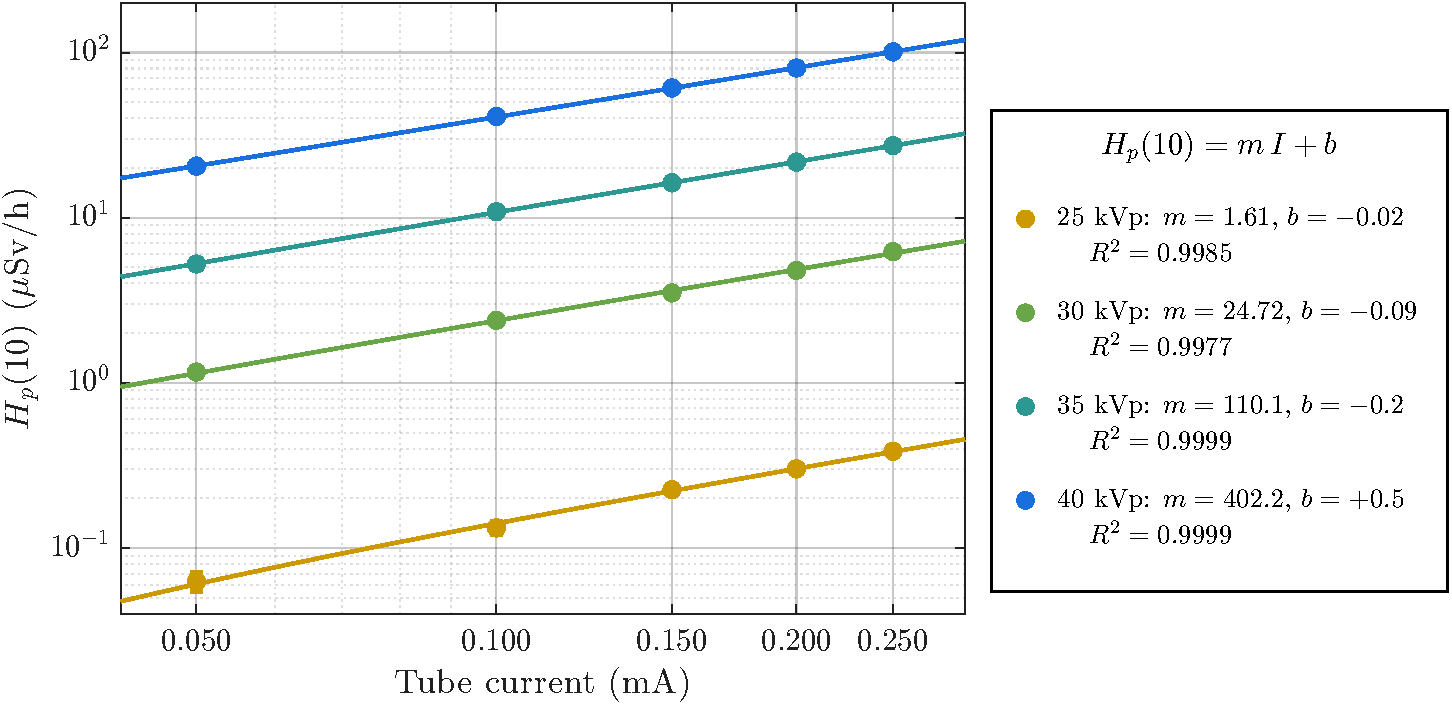
\includegraphics[width=1\linewidth]{images/dose_rate_linearity.pdf}
  \caption[Reconstructed $H_p(10)$ rate as a function of tube current.]{Reconstructed $H_p(10)$ rate as a function of tube current, for tube
potentials of 25-40~kVp and currents of 0.050-0.250~mA.
  }
  \label{fig:dose_linearity}
\end{figure}

The measurements span 0.063 to 101~$\mu$Sv/h. At every tube potential the dose rate increases linearly with the tube current, with $R^2 \geq 0.998$. The fitted intercepts are consistent with zero at all four potentials, as expected, since no tube current means no counts and therefore no dose. The largest deviation from the fitted line is $6\%$, occurring at 25~kVp, and is attributed to the poorer counting statistics at this potential. The total count rate over the whole set ranges from 82 to $1.9\times10^{3}$~s$^{-1}$, against the saturation count rate of $56\times10^{3}$~s$^{-1}$ given in Section~\ref{sec:pulse_sampling}. The measurements therefore lie within a reliable photon counting region, where dead time and pile-up are negligible. The ratio $N_2/N_1$ remains constant with the tube current at the potentials where both bins are populated, indicating that the distribution of counts is preserved over this range. 

The relevance of this range can be assessed against the isodose map of Fig.~\ref{fig:scatter}, keeping in mind that the reliability of the reconstructed values depends on the assumptions of the dose calibration described in the previous section. That map spans 0.0075 to 167~$\mu$Sv/h behind a lead apron and 0.5 to $12\times10^{3}$~$\mu$Sv/h without one, at chest level, for one of the most demanding procedures in this modality. The range reconstructed here overlaps most of the shielded scale, but covers only the lower part of the unshielded one, which are detected at higher scattering distances. Other studies report average dose rates of approximately 30~$\mu$Sv/h for conventional interventions above personal shielding~\cite{53}. The dose rates are therefore relevant, but the position at which the dosimeter is worn should be considered when a full energy and dose calibration is defined. The limit in count rate has also not been established, and the performance of the prototype has to be characterised before an operating range in dose rate can be claimed. Reaching those rates would involve higher photon energies, and establishing the limit of linearity requires, once again, a more complete energy and dose calibration.








